\section{Métodos}
\subsection{Modalidad de la investigación}
En la siguiente sección se detalla la modalidad de la investigación que se aplicara al desarrollo de este proyecto.
\bigbreak
\textbf{Investigación bibliográfica} \\
Debido a que se requiere de una exploración previa de investigaciones relacionadas para poder identificar las similitudes y diferencias con el presente proyecto, se utilizará la investigación bibliográfica.
\bigbreak
\textbf{Investigación cuantitativa} \\
Debido a que se aplicarán encuestas para la recolección de datos que posteriormente serán analizados mediante métodos estadísticos, se utilizará la investigación cuantitativa.

\subsection{Población y muestra}\label{subsec:poblacion}

Para el sistema web administrativo se considerará como población a los 4 miembros de la directiva del conjunto habitacional {\textquotedblleft}El Portal de la Viña{\textquotedblright}.\\

Para el sistema móvil se considerará como población a un solo propietario de cada residencia del conjunto habitacional {\textquotedblleft}El Portal de la Viña{\textquotedblright}, teniendo un total de 303 propietarios. Del cual se tomara la siguiente muestra:

\bigbreak
\textbf{Muestra}
\begin{itemize}
    \item n = tamaño de la muestra.
    \item N = tamaño de la población (303).
    \item Z = nivel de confianza (1.96).
    \item d = desviación estándar (0.5).
    \item e = error de estimación máximo aceptable (0.09).
\end{itemize}
\begin{equation}
    \label{eq:equation}
    n = \frac{N * Z^2 * d * (1-d)}{e^2 * (N-1) + Z^2 * d * (1-d)}
\end{equation}
\begin{equation}
    \label{eq:equation1}
    n = \frac{303 * 1.96^2 * 0.5 * (1-0.5)}{0.09^2 * (303-1) + 1.96^2 * 0.5 * (1-0.5)}
\end{equation}
\begin{equation}
    \label{eq:equation2}
    n = 85.22
\end{equation}

De las 303 casas con un nivel de confianza del 95\% y un error de estimación del 9\% se obtiene una muestra de 85 casas.

\subsection{Recolección de información}

La información se recolectó mediante el uso de encuestas y entrevistas. Las encuestas fueron aplicadas a los propietarios del conjunto habitacional {\textquotedblleft}El Portal de la Viña{\textquotedblright} para determinar necesidades y posteriormente medir la usabilidad de los sistemas informáticos propuestos en la presente investigación. Las entrevistas fueron aplicadas a los miembros de la directiva del conjunto habitacional {\textquotedblleft}El Portal de la Viña{\textquotedblright} para obtener información técnica y legal del conjunto habitacional.
\bigbreak
Las siguientes respuestas son interpretaciones de las entrevistas realizadas a los miembros de la directiva del conjunto habitacional {\textquotedblleft}El Portal de la Viña{\textquotedblright} por lo cual no son transcripciones literales de las respuestas dadas por los entrevistados.

%\begin{table}
%    \centering
%    \caption{Entrevista a la directiva del conjunto habitacional {\textquotedblleft}El Portal de la Viña{\textquotedblright}}
\newpage
\begin{center}
    \begin{small}

    \begin{longtable}[c]{|p{0.15\textwidth} |p{0.4\textwidth} |p{0.37\textwidth}|}
        \caption{Entrevista a la directiva del conjunto habitacional {\textquotedblleft}El Portal de la Viña{\textquotedblright}}\\
        \hline
        \textbf{N. Pregunta} & \textbf{Respuesta} & \textbf{Observación}\\
        \hline
            1. & Las funciones de la directiva son mayormente administrativas y económicas en donde la presidencia(presidente y vicepresidente) se encargan de gestionar las multas, los eventos sociales y de asambleas, extender comunicados, gestionar las normativas y gestionar los parqueaderos.
            La tesorería se encarga de gestionar los ingresos y egresos del conjunto mediante el uso de hojas de cálculo como Excel, en donde los ingresos están dados por los pagos que se realizan por parte de los propietarios tales como las alícuotas, los parqueaderos y las multas.
            Los egresos, por otro lado, están dados por los pagos de los servicios que se tiene contratado para el condominio tales como la limpieza, jardinería, guardias y otros servicios adicionales.
            También se encarga de extender los recibos de pagos los cuales pueden ser pagados en efectivo o mediante una transferencia bancaria.
            Además, en tesorería se lleva el control de los horarios de cortes de jardín y de limpieza de áreas comunes.
            En secretaría se encarga de elaborar las actas de asamblea, informes de asistencia en las asambleas e invitaciones a los eventos sociales.
            & Se evidencia una gran carga de trabajo en tesorería, ya que es únicamente una persona la que debe atender a las 303 casas.
            También el hecho de tener todos los registros de ingresos y egresos en hojas de cálculo son un problema para la directiva, porque dificulta la búsqueda de information y la generación de reportes.
            Adicionalmente, el presidente para poder gestionar los parqueaderos se basa en un croquis de los mismos para poder identificarlos, lo cual es un proceso lento y tedioso.\\
        \hline
        2. & El presidente tiene como función extra realizar mínimo una ronda de revisiones de las áreas comunes del conjunto para encontrar fallas y poder realizar mejoras.
        La tesorera tiene como iniciativa estar al pendiente de las novedades que ocurran en guardianía.
       La secretaria tuvo como iniciativa realizar un seguimiento de las actividades diarias que realizan la directiva.
       & Estas funciones adicionales serán agregadas al sistema para que se introduzcan en el modelo de gestión del conjunto habitacional.\\
        \hline
        3. & La presidencia entrega certificados de no adeudamiento a los propietarios que lo soliciten, comunicados de eventos y asambleas y notificaciones de multas.
        La tesorería entrega los recibos de pagos, reporte de cartera de los parqueaderos de zona azul y emisión de listados de suspension de corte de jardín.
       La secretaría entrega las actas de asamblea y los informes de asistencia.
        & Se evidenció la necesidad de la directiva de poder digitalizar y generar gran parte de los documentos mencionados\\
        \hline
        4. & Presentar el físico cédula y papeleta de votación junto con sus respetivas copias, Predio o escrituras de la casa y firmar una acta de compromiso.
        & Este proceso al depender de documentos físicos los cuales no pueden ser enviados por medios digitales se mantendrán de la misma forma, sin embargo, se sistematizara el proceso para asignar el cambio de propietario de cada parqueadero.\\
        \hline
        5. & Se utiliza un croquis que está en guardianía y también se usa como guía la numeración de la casa que tiene en frente.
        & Esta forma que tienen de identificar no es eficiente, ya que no todas las casas del conjunto tienen domicilios en frente lo cual se optara por colocar un código de enumeración en cada parqueadero dependiendo de a que grupo pertenezcan.\\
        \hline
        6. & A todos los servicios que se quieren contratar se solicita una proforma y de acuerdo a los planes que ofrezcan se elige el que más se ajuste a las necesidades del conjunto.
        & Los servicios que se contratan se registran en una hoja de cálculo siendo así un proceso manual y tedioso, por lo cual se optara por digitalizar este proceso.\\
        \hline
        7. & No se lleva contabilidad como tal sino que se lleva un registro de ingresos y egresos.
        Los reportes varían dependiendo de la necesidad de la directiva, ya que no se tiene un reporte fijo salvo la rendición de cuentas que se realiza en las asambleas.
        & Se solicitó por parte de la directiva establecer unos reportes fijos que se generen automáticamente y que sean de fácil acceso.\\
        \hline
        8. & Se utiliza la pizarra de guardianía para emitir comunicados y también se endian mensajes por WhatsApp.
        & La directiva menciona que estos medios no son eficientes debido a que si el comunicado es enviado por WhatsApp muchos propietarios no lo reciben, ya que los grupos se llenan de mensajes que no son relevantes y discusiones entre vecinos.
        Por otro lado, la pizarra de guardianía no suele ser vista por todos los propietarios, debido a que han existido quejas que cuesta mucho leer lo que se escribe en ella.\\
        \hline
        9. & El registro de asistencias se hace en una hoja impresa en la cual se coloca el nombre del propietario o inquilino, el número de casa y la firma.
        Mientras que para el conteo de votos se realiza mediante el conteo de manos alzadas.
        & Se evidencia una necesidad clara de poder agilizar el proceso de registro de asistencia y el conteo de votaciones.\\
        \hline
        10.
        & Se le multa al residente por su inasistencia injustificada, ya que se le dan tres días para justificarla.
        & Ocasionalmente, suelen faltar más de veinte propietarios a las asambleas y se debe multar a todos ellos, lo cual es un proceso tedioso debido a que se les debe notificar uno por uno y esto consume mucho tiempo.\\
        \hline
        11.
        & Actualmente el registro de pagos y la generación de recibos son manuales y esto ha ocasionado quejas en los propietarios, ya que no se les entrega el recibo de pago a tiempo.
        Durante las asambleas la asistencia lleva más de media hora en concluirse.
        & La necesidad de poder sistematizar los pagos y la generación de recibos es evidente por parte de la directiva, así como también la necesidad de agilizar el proceso de registro de asistencia.\\
        \hline
        12.
        & El buzón de sugerencias es muy poco utilizado por los propietarios.
        & El buzón es elemento importante para la directiva, ya que las quejas las reciben a sus numerous de teléfono personal y esto les ocasiona que a menudo que no puedan atender todos o se les pase por alto alguno de estos mensajes.\\
        \hline
        13.
        & Casi toda la información que se maneja en la directiva están en libros escritos a mano y en hojas de cálculo.
        & Estos libros y hojas de cálculo se han ido pasando de directiva en directiva y ocasionalmente se pierden o se dañan y en los peores casos han provocado malos entendidos\\
        \hline
    \end{longtable}
    \end{small}
\end{center}
%\end{table}

%\subsubsection{Validación del instrumento}
%\begin{itemize}
%    \item Alfa de Cronbach.
%    Con la finalidad de evaluar la consistencia interna de las preguntas del cuestionario se utilizó el coeficiente de alfa de Cronbach con los datos recolectados de las preguntas 1,2,3,4,6,7 y 8 dirigidas a los propietarios del conjunto habitacional {\textquotedblleft}El Portal de la Viña{\textquotedblright}(Véase el Anexo), las cuales fueron planteadas mediante una escala de Likert de 5 puntos.
%    Para su cálculo se empleó la siguiente ecuación:
%    \begin{equation}
%        \label{eq:equation3}
%        \alpha = \frac{k}{{k - 1}} \left(1 - \frac{{\sum_{i=1}^{k} \sigma_{i}^{2}}}{{\sigma_{T}^{2}}} \right)
%    \end{equation}
%
%    Donde:
%    \begin{itemize}
%        \item $\alpha$ = Coeficiente de alfa de Cronbach.
%        \item $k$ = Número de ítems.
%        \item $\sigma_{i}^{2}$ = Varianza de cada ítem.
%        \item $\sigma_{T}^{2}$ = Varianza total.
%    \end{itemize}
%    Para el cáculo del mismo se utilizó una hoja de Excel para facilitar su cálculo(Véase Anexo\ref{app:alfa-cronbach-excel}), obteniendo un valor de 0.35, lo cual indica que el cuestionario es poco confiable o nulo.
%
%\end{itemize}
\newpage
\subsubsection{Resultados de la encuesta aplicada a los residentes del conjunto habitacional {\textquotedblleft}El Portal de la Viña{\textquotedblright}}
\textbf{Pregunta 1:} ¿Cree usted que el proceso actual para obtener la información de las obligaciones financieras (pagos, multas, etc.) de su domicilio es eficiente?
    \begin{table}[H]
        \centering
        \caption{Resultados de la pregunta uno}
        \begin{tabular}{|c|c|c|}
            \hline
            \textbf{Indicador} & \textbf{Frecuencia} &  \textbf{Porcentaje} \\
            \hline
            Totalmente de acuerdo & 47 & 31.5\% \\
            \hline
            De acuerdo & 61 & 40.9\% \\
            \hline
            Ni de acuerdo ni en desacuerdo & 23 & 15.4\% \\
            \hline
            En desacuerdo & 13 & 8.7\% \\
            \hline
            Totalmente en desacuerdo & 5 & 3.5\% \\
            \hline
            \textbf{Suma total} & 149 & 100\% \\
            \hline
        \end{tabular}\label{tab:table}
    \end{table}
    \begin{figure}[H]
              \centering
              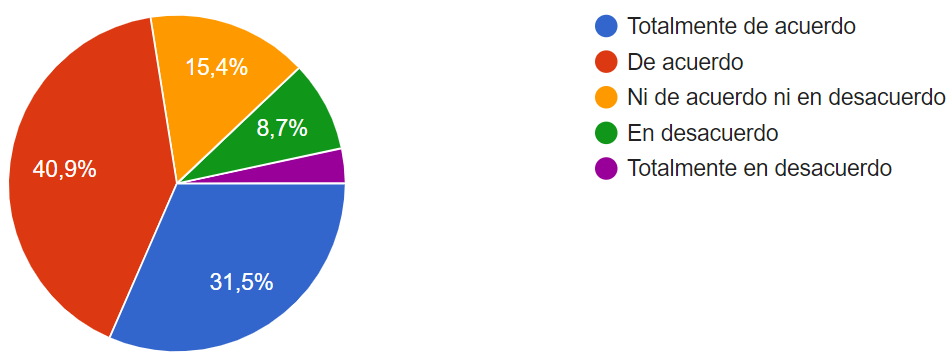
\includegraphics[width=0.8\textwidth]{resources/images/p1}
              \caption{Resultados de la encuesta en la pregunta uno}\label{fig:figure_p1}
    \end{figure}

\textbf{Análisis e interpretación:}\\
Los resultados de la pregunta uno muestran que el 31.5\% de los propietarios del conjunto habitacional {\textquotedblleft}El Portal de la Viña{\textquotedblright} están totalmente de acuerdo con el proceso actual para obtener la información de las obligaciones financieras de su domicilio, el 40.9\% de los propietarios están de acuerdo con el proceso actual, el 15.4\% de los propietarios ni están de acuerdo ni en desacuerdo con el proceso actual, el 8.7\% de los propietarios están en desacuerdo con el proceso actual y por último el 3.5\% de los propietarios están totalmente en desacuerdo con el proceso actual.
Tomando en cuenta los resultados obtenidos en la encuesta, se puede observar que el 72.4\% de los propietarios del conjunto habitacional consideran que el proceso actual para obtener la información de las obligaciones financieras de su domicilio es eficiente, mientras que, el 27.6\% de los propietarios consideran que el proceso actual no es eficiente y tomando en consideración las entrevistas realizadas a tesorería se concluye que se puede agilizar el proceso de consulta de información mediante el uso de una aplicación móvil.
\bigbreak

\textbf{Pregunta 2:} ¿Con que frecuencia solicita la información de las obligaciones financieras (pagos, multas, etc.) de su domicilio a tesorería?
    \begin{table}[H]
              \centering
              \caption{Resultados de la pregunta dos}
              \begin{tabular}{|c|c|c|}
                  \hline
                  \textbf{Indicador} & \textbf{Frecuencia} &  \textbf{Porcentaje} \\
                  \hline
                  Por lo menos una vez al mes & 135 & 90.6\% \\
                  \hline
                  Dos veces al mes & 5 & 3.4\% \\
                  \hline
                  Tres veces al mes
                  & 5 & 3.4\% \\
                  \hline
                  Cuatro veces al mes & 0 & 0\% \\
                  \hline
                  Más de cuatro veces al mes & 4 & 2.7\% \\
                  \hline
                  \textbf{Suma total} & 149 & 100\% \\
                  \hline
              \end{tabular}\label{tab:table_preg_2}
    \end{table}
    \begin{figure}[H]
              \centering
              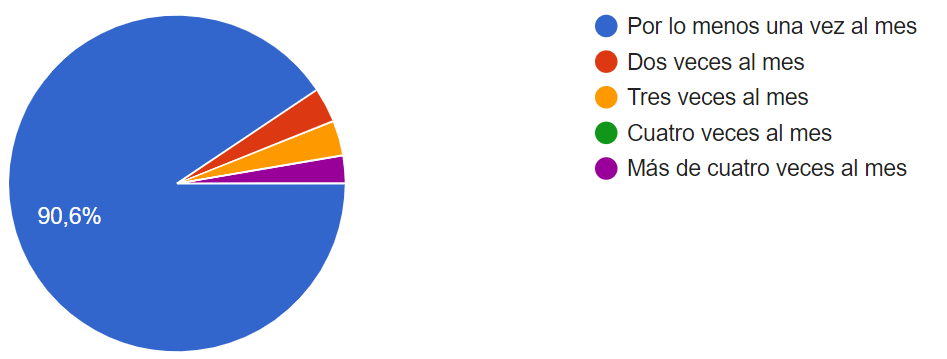
\includegraphics[width=0.8\textwidth]{resources/images/p2}
              \caption{Resultados de la encuesta en la pregunta dos}\label{fig:figure_p2}
    \end{figure}

\textbf{Análisis e interpretación:}\\
Los resultados de la pregunta dos evidencian que el 90.6\% de los propietarios del conjunto habitacional {\textquotedblleft}El Portal de la Viña{\textquotedblright} solicitan por lo menos una vez al mes la información de las obligaciones financieras de su domicilio a tesorería, el 3.4\% de los propietarios solicitan dos veces al mes, el 3.4\% de los propietarios solicitan tres veces al mes, el 0\% de los propietarios solicitan cuatro veces al mes y por último el 2.7\% de los propietarios solicitan más de cuatro veces al mes.
Por tanto, se puede observar que existe una demanda considerable de solicitudes a tesorería de manera mensual, lo cual junto con la entrevista realizada a tesorería se concluye que se puede facilitar el proceso de consulta de información mediante el uso de una aplicación móvil.

\bigbreak
\textbf{Pregunta 3:} ¿Cree usted que el proceso actual para el registro de asistencias durante la asamblea es eficiente en términos de tiempo?
    \begin{table}[H]
        \centering
        \caption{Resultados de la pregunta tres}
        \begin{tabular}{|c|c|c|}
            \hline
            \textbf{Indicador} & \textbf{Frecuencia} &  \textbf{Porcentaje} \\
            \hline
            Totalmente de acuerdo & 29 & 19.5\% \\
            \hline
            De acuerdo & 55 & 36.9\% \\
            \hline
            Ni de acuerdo ni en desacuerdo & 34 & 22.8\% \\
            \hline
            En desacuerdo & 17 & 11.4\% \\
            \hline
            Totalmente en desacuerdo & 14 & 9.4\% \\
            \hline
            \textbf{Suma total} & 149 & 100\% \\
            \hline
        \end{tabular}\label{tab:table_preg_3}
    \end{table}
    \begin{figure}[H]
        \centering
        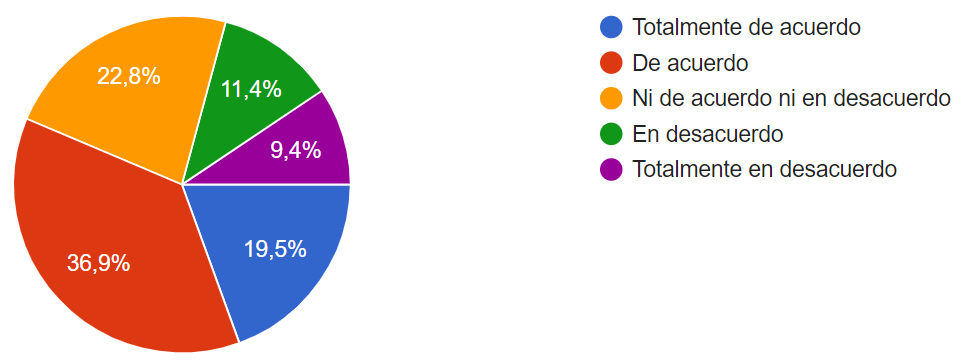
\includegraphics[width=0.8\textwidth]{resources/images/p3}
        \caption{Resultados de la encuesta en la pregunta tres}\label{fig:figure_p3}
    \end{figure}

\textbf{Análisis e interpretación:}\\
Los resultados de la pregunta tres muestran que el 19.5\% de los propietarios del conjunto habitacional {\textquotedblleft}El Portal de la Viña{\textquotedblright} están totalmente de acuerdo con el proceso actual para el registro de asistencias durante la asamblea, el 36.9\% de los propietarios están de acuerdo con el proceso actual, el 22.8\% de los propietarios ni están de acuerdo ni en desacuerdo con el proceso actual, el 11.4\% de los propietarios están en desacuerdo con el proceso actual y por último el 9.4\% de los propietarios están totalmente en desacuerdo con el proceso actual.
Por lo tanto, se observa que el 56.4\% de los propietarios del conjunto habitacional consideran que el proceso actual para el registro de asistencias durante la asamblea es eficiente en términos de tiempo, mientras que el 43.6\% de los propietarios consideran que el proceso actual no es eficiente y tomando en consideración las entrevistas realizadas a presidencia se concluye que se puede optimizar el proceso de registro de asistencias mediante el uso de sistemas informáticos.
\bigbreak
\textbf{Pregunta 4:} ¿Considera usted que el conteo actual de las votaciones durante las asambleas es transparente y eficiente?
    \begin{table}[H]
        \centering
        \caption{Resultados de la pregunta cuatro}
        \begin{tabular}{|c|c|c|}
            \hline
            \textbf{Indicador} & \textbf{Frecuencia} &  \textbf{Porcentaje} \\
            \hline
            Totalmente de acuerdo & 50 & 33.6\% \\
            \hline
            De acuerdo & 57 & 38.3\% \\
            \hline
            Ni de acuerdo ni en desacuerdo & 31 & 20.8\% \\
            \hline
            En desacuerdo & 5 & 3.4\% \\
            \hline
            Totalmente en desacuerdo & 6 & 4\% \\
            \hline
            \textbf{Suma total} & 149 & 100\% \\
            \hline
        \end{tabular}\label{tab:table_preg_4}
    \end{table}
    \begin{figure}[H]
        \centering
        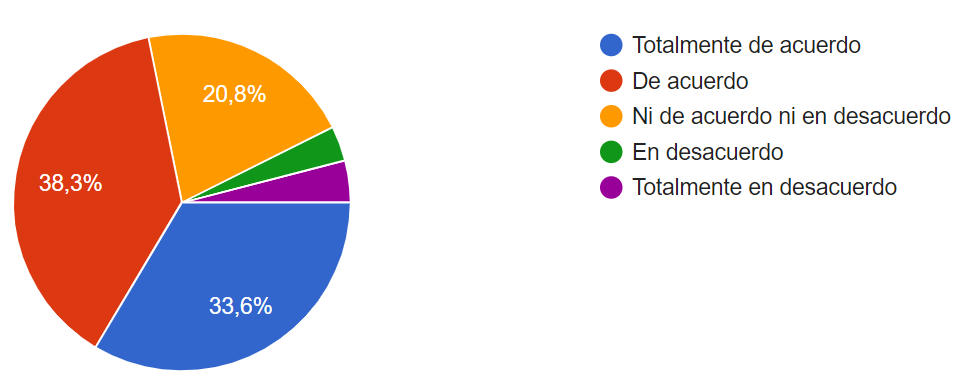
\includegraphics[width=0.8\textwidth]{resources/images/p4}
        \caption{Resultados de la encuesta en la pregunta cuatro}\label{fig:figure_p4}
    \end{figure}

\textbf{Análisis e interpretación:}\\
Los resultados de la pregunta cuatro muestran que el 33.6\% de los propietarios del conjunto habitacional {\textquotedblleft}El Portal de la Viña{\textquotedblright} están totalmente de acuerdo con el conteo actual de las votaciones durante las asambleas, el 38.3\% de los propietarios están de acuerdo con el conteo actual, el 20.8\% de los propietarios ni están de acuerdo ni en desacuerdo con el conteo actual, el 3.4\% de los propietarios están en desacuerdo con el conteo actual y por último el 4\% de los propietarios están totalmente en desacuerdo con el conteo actual.
Por lo cual, se puede observar que el 71.9\% de los propietarios del conjunto habitacional consideran que el conteo actual de las votaciones durante las asambleas es transparente y eficiente, mientras que el 28.1\% de los propietarios consideran que el conteo actual no es transparente y eficiente y tomando en consideración las entrevistas realizadas a presidencia en donde se expuso que la duración de las mismas suelen ser de entre veinte a treinta minutos, se concluye que se puede sistematizar el proceso de conteo de votaciones mediante el uso de sistemas informáticos para reducir y cumplir así con los tiempos establecidos de duración de las asambleas.
\bigbreak
\textbf{Pregunta 5:} ¿Ha experimentado retrasos en la entrega de los comprobantes de pagos?
    \begin{table}[H]
        \centering
        \caption{Resultados de la pregunta cinco}
        \begin{tabular}{|c|c|c|}
            \hline
            \textbf{Indicador} & \textbf{Frecuencia} &  \textbf{Porcentaje} \\
            \hline
            Si & 62 & 41.6\% \\
            \hline
            No & 87 & 58.4\% \\
            \hline
            \textbf{Suma total} & 149 & 100\% \\
            \hline
        \end{tabular}\label{tab:table_preg_5}
    \end{table}
    \begin{figure}[H]
        \centering
        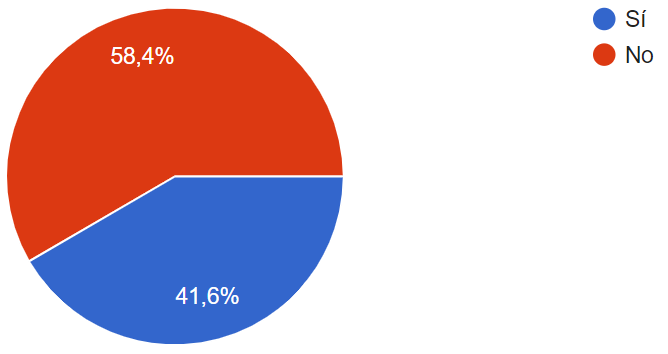
\includegraphics[width=0.8\textwidth]{resources/images/p5}
        \caption{Resultados de la encuesta en la pregunta cinco}\label{fig:figure_p5}
    \end{figure}

\textbf{Análisis e interpretación:}\\
Los resultados de la pregunta cinco muestran que el 41.6\% de los propietarios del conjunto habitacional {\textquotedblleft}El Portal de la Viña{\textquotedblright} han experimentado retrasos en la entrega de los comprobantes de pagos, mientras que el 58.4\% de los propietarios no han experimentado retrasos en la entrega de los comprobantes de pagos.
Por tanto, se evidencia que un sistema informático administrativo puede ser de gran ayuda para la directiva del conjunto habitacional, ya que se puede sistematizar el proceso de entrega de comprobantes de pagos y evitar retrasos en la entrega de los mismos.
\bigbreak
\textbf{Pregunta 6:} ¿Con qué frecuencia olvida que el pago de alícuotas de su domicilio esta por vencer?
    \begin{table}[H]
        \centering
        \caption{Resultados de la pregunta seis}
        \begin{tabular}{|c|c|c|}
            \hline
            \textbf{Indicador} & \textbf{Frecuencia} &  \textbf{Porcentaje} \\
            \hline
            Muy frecuentemente & 21 & 14.1\% \\
            \hline
            Frecuentemente & 20 & 13.4\% \\
            \hline
            Ocasionalmente & 31 & 20.8\% \\
            \hline
            Raramente & 36 & 24.2\% \\
            \hline
            Nunca & 41 & 27.5\% \\
            \hline
            \textbf{Suma total} & 149 & 100\% \\
            \hline
        \end{tabular}\label{tab:table_preg_6}
    \end{table}
    \begin{figure}[H]
        \centering
        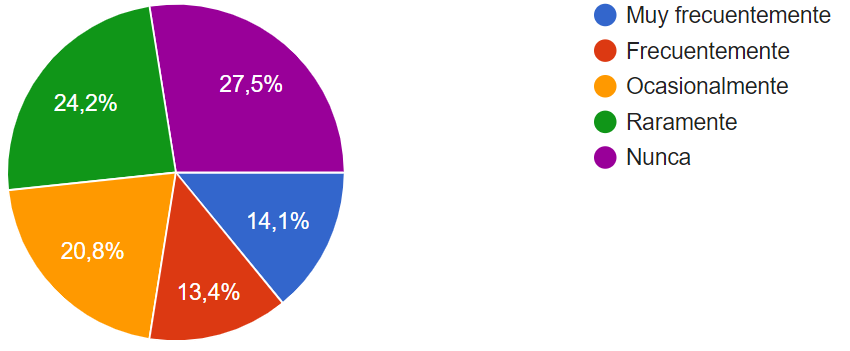
\includegraphics[width=0.8\textwidth]{resources/images/p6}
        \caption{Resultados de la encuesta en la pregunta seis}\label{fig:figure_p6}
    \end{figure}

\textbf{Análisis e interpretación:}\\
Los resultados de la pregunta seis muestran que el 14.1\% de los propietarios del conjunto habitacional {\textquotedblleft}El Portal de la Viña{\textquotedblright} olvidan muy frecuentemente que el pago de alícuotas de su domicilio están por vencer, el 13.4\% de los propietarios olvidan frecuentemente, el 20.8\% de los propietarios olvidan ocasionalmente, el 24.2\% de los propietarios olvidan raramente y por último el 27.5\% de los propietarios nunca olvidan que el pago de alícuotas.
Para mejorar estos resultados se puede implementar recordatorios de pagos por vencer mediante una aplicación móvil, ya que se evidencia que el 48.3\% de los propietarios lo olvidan muy frecuentemente, frecuentemente u ocasionalmente.
\bigbreak
\textbf{Pregunta 7:} ¿Con qué frecuencia ha utilizado el buzón de quejas/sugerencias?
    \begin{table}[H]
        \centering
        \caption{Resultados de la pregunta siete}
        \begin{tabular}{|c|c|c|}
            \hline
            \textbf{Indicador} & \textbf{Frecuencia} &  \textbf{Porcentaje} \\
            \hline
            Nunca lo he usado & 142 & 95.3\% \\
            \hline
            Al menos una vez al mes & 6 & 4\% \\
            \hline
            Dos veces al mes & 0 & 0\% \\
            \hline
            Tres veces al mes & 0 & 0\% \\
            \hline
            Más de tres veces al mes & 1 & 0.7\% \\
            \hline
            \textbf{Suma total} & 149 & 100\% \\
            \hline
        \end{tabular}\label{tab:table_preg_7}
    \end{table}
    \begin{figure}[H]
        \centering
        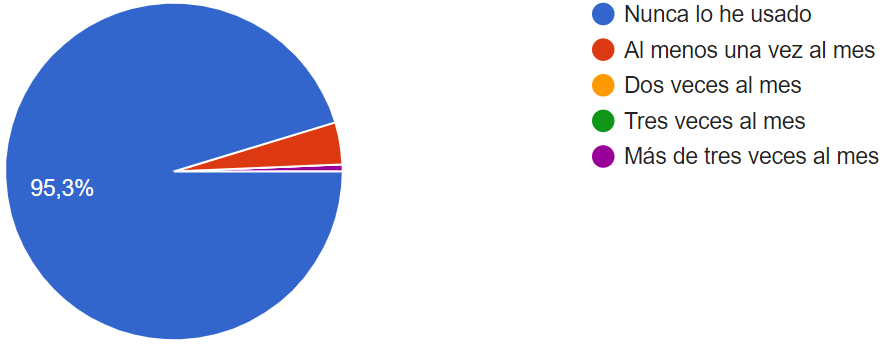
\includegraphics[width=0.8\textwidth]{resources/images/p7}
        \caption{Resultados de la encuesta en la pregunta siete}\label{fig:figure_p7}
    \end{figure}

\textbf{Análisis e interpretación:}\\
Los resultados de la pregunta siete muestran que el 95.3\% de los propietarios del conjunto habitacional {\textquotedblleft}El Portal de la Viña{\textquotedblright} nunca han utilizado el buzón de quejas/sugerencias, el 4\% de los propietarios lo han utilizado al menos una vez al mes, el 0\% de los propietarios lo han utilizado dos veces al mes, el 0\% de los propietarios lo han utilizado tres veces al mes y por último el 0.7\% de los propietarios lo han utilizado más de tres veces al mes.
Por tanto, se evidencia que el buzón de quejas/sugerencias no es utilizado por los propietarios del conjunto habitacional, lo cual se puede mejorar mediante una aplicación móvil que permita a los propietarios enviar sus quejas y sugerencias de una manera más sencilla y eficiente.
\bigbreak
\textbf{Pregunta 8:} ¿Considera usted que los medios actuales (WhatsApp/pizarrón en la garita) que utiliza la directiva para publicar comunicados son eficientes?

    \begin{table}[H]
        \centering
        \caption{Resultados de la pregunta ocho}
        \begin{tabular}{|c|c|c|}
            \hline
            \textbf{Indicador} & \textbf{Frecuencia} &  \textbf{Porcentaje} \\
            \hline
            Totalmente de acuerdo & 58 & 38.9\% \\
            \hline
            De acuerdo & 68 & 45.6\% \\
            \hline
            Ni de acuerdo ni en desacuerdo & 12 & 8.1\% \\
            \hline
            En desacuerdo & 4 & 2.7\% \\
            \hline
            Totalmente en desacuerdo & 7 & 4.7\% \\
            \hline
            \textbf{Suma total} & 149 & 100\% \\
            \hline
        \end{tabular}\label{tab:table_preg_8}
    \end{table}
    \begin{figure}[H]
        \centering
        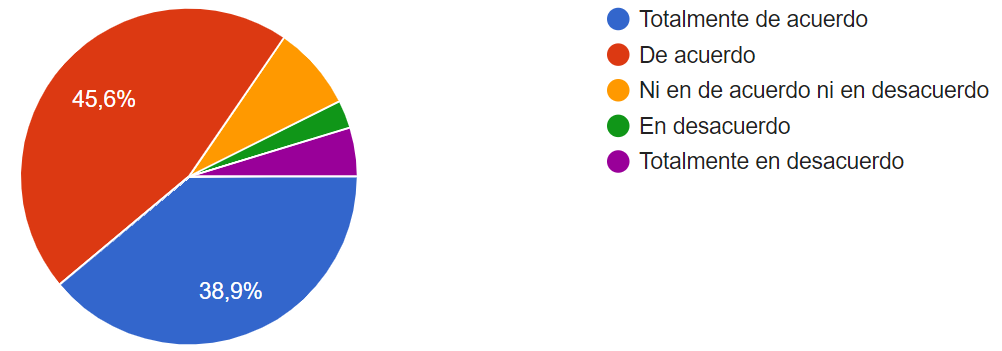
\includegraphics[width=0.8\textwidth]{resources/images/p8}
        \caption{Resultados de la encuesta en la pregunta ocho}\label{fig:figure_p8}
    \end{figure}

\textbf{Análisis e interpretación:}\\
Los resultados de la pregunta ocho muestran que el 38.9\% de los propietarios del conjunto habitacional {\textquotedblleft}El Portal de la Viña{\textquotedblright} están totalmente de acuerdo con los medios actuales que utiliza la directiva para publicar comunicados, el 45.6\% de los propietarios están de acuerdo con los medios actuales, el 8.1\% de los propietarios ni están de acuerdo ni en desacuerdo con los medios actuales, el 2.7\% de los propietarios están en desacuerdo con los medios actuales y por último el 4.7\% de los propietarios están totalmente en desacuerdo con los medios actuales.
Para mejorar estos resultados se puede implementar un sistema informático que permita a la directiva publicar comunicados de una manera más centralizada, ya que tomando en consideración las entrevistas realizadas a la directiva el uso de WhatsApp no es apto para la publicación de comunicados por el mal uso que le dan los demás residentes y el pizarrón en la garita no es visible para todos los propietarios.
\bigbreak
\textbf{Pregunta 9:} ¿Preferiría utilizar una aplicación móvil que le permita revisar la información de las obligaciones financieras de su domicilio, el registro de su asistencia y voto durante las asambleas, se le envíen notificaciones recordándole los pagos por vencer o que ha sido multado por alguna infracción?
    \begin{table}[H]
        \centering
        \caption{Resultados de la pregunta nueve}
        \begin{tabular}{|c|c|c|}
            \hline
            \textbf{Indicador} & \textbf{Frecuencia} &  \textbf{Porcentaje} \\
            \hline
            Si & 127 & 85.2\% \\
            \hline
            No & 22 & 14.8\% \\
            \hline
            \textbf{Suma total} & 149 & 100\% \\
            \hline
        \end{tabular}\label{tab:table_preg_9}
    \end{table}
    \begin{figure}[H]
        \centering
        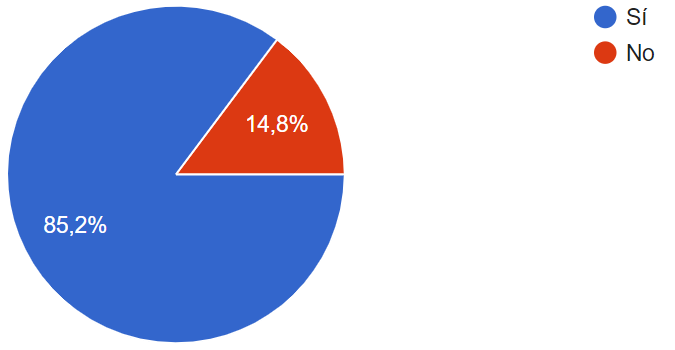
\includegraphics[width=0.8\textwidth]{resources/images/p9}
        \caption{Resultados de la encuesta en la pregunta nueve}\label{fig:figure_p9}
    \end{figure}

\textbf{Análisis e interpretación:}\\
Los resultados de la pregunta nueve muestran que el 85.2\% de los propietarios del conjunto habitacional {\textquotedblleft}El Portal de la Viña{\textquotedblright} preferirían utilizar una aplicación móvil que les permita revisar la información de las obligaciones financieras de su domicilio, el registro de su asistencia y voto durante las asambleas, se les envíen notificaciones recordándoles los pagos por vencer o que han sido multados por alguna infracción, mientras que el 14.8\% de los propietarios no preferirían utilizar una aplicación móvil.


\subsection{Procesamiento y análisis de datos}\label{subsec:procesamiento-y-analisis-de-datos}

Con la información recolectada a través de las entrevistas y las encuestas se concluyó que:
\begin{itemize}
    \item Actualmente la directiva lleva mucho de sus procesos de forma manual o en hojas de cálculo que han ocasionado atrasos y una alta carga de trabajo para todos los miembros de la misma.
    Los procesos administrativos actualmente funcionan, pero no son eficientes.
    Cada uno de los miembros de la directiva tienen sus funciones específicas, pero no cuentan con un sistema que les permita realizarlos de una manera más sencilla, puesto que todos ellos tienen empleos y no pueden dedicarle todo el tiempo que quisieran al conjunto habitacional.
    \item En presidencia se lleva a cabo el control y manejo de los parqueaderos de una manera manual y muy tediosa, debido a que deben de dibujar un croquis manual de los parqueaderos y actualizar las hojas de excel con los datos de los propietarios. El tiempo empleado en las asambleas es demasiado extenso, por el motivo de que se debe hacer el registro de asistencia por cada residente de manera manual en una hoja impresa.
    \item En tesorería se maneja la información económica del conjunto en hojas de cálculo, teniendo en cuenta que son 303 casas y 275 parqueaderos en total, se convierte en un problema muy alto en cuanto a la cantidad de información que se debe manejar y el tiempo que se debe emplear en la generación de reportes. Además lo anteriormente mencionado provoca atrasos en la entrega de recibos de pagos.
    \item En secretaría se lleva la generación de gran parte de actas y convocatorías mediante el uso de Word o Canva, en donde se identificó que estos documentos son generados de forma manual y para emitirlos se utiliza WhatsApp. Como consecuencía de esto los propietarios no suelen enterarse de las convocatorías ya que el grupo de  WhatsApp esta en gran parte del tiempo con mensajes irrelevantes y discusiones entre vecinos.
    \item De las encuestas realizadas a los propietarios se pudo identificar que la mayoría están conformes con la gestión de la directiva, sin embargo, se
     evidenció que los atrasos en las entregas de recibos de pagos es un problema bastante común. También existe un poco uso del buzón de sugerencias, ya que los propietarios prefieren comunicarse directamente con los miembros de la directiva. Y por último existe una necesidad alta de poder tener una aplicación móvil que les permite consultar información de su domicilio y notificar de eventos importantes.
\end{itemize}